
                \begin{figure}
                    \centering
                    \begin{tikzpicture}
                        \pgfplotsset{%
                            width=1\textwidth,
                            height=0.5\textheight
                        }
                        \begin{axis}[
                            xlabel={Start battery level},
                            ylabel={Average dynamic energy (watt)},
                            ymin=0,ymax=20,
                        ]
                        
                            \addplot [mark=none, ultra thick, red]  coordinates {
                            (40, 13.743050207605922)(45, 13.995216125365774)(50, 14.3366422723928)(55, 13.861328803676027)(60, 13.9520544253169)(65, 13.607897859860785)(70, 13.661217957402677)(75, 13.83989770460602)(80, 12.454305913583585)
                            };
                            \addlegendentry{Surface4Pro - IntelPowerGadget}
                            
                            \addplot [mark=none, ultra thick, blue]  coordinates {
                            (40, 12.451889106121774)(45, 12.688939452739993)(50, 12.669787358985896)(55, 12.690882453354114)(60, 12.587299079607842)(65, 12.629570181025164)(70, 12.731095231850171)(75, 12.479387800802002)(80, 11.932915888199908)
                            };
                            \addlegendentry{Surface4Pro - HardwareMonitor}
                            
                            \addplot [mark=none, ultra thick, orange]  coordinates {
                            (45, 7.258815908797952)(50, 7.26610619968319)(55, 7.26687449118181)(60, 7.266766074518518)(65, 7.268291213450709)(70, 7.279337122021078)(75, 7.302825434955896)(80, 7.152999552327533)
                            };
                            \addlegendentry{Surface4Pro - RAPL}
                            
                            \addplot [mark=none, dashdotted, red]  coordinates {
                            (40, 7.961305351670973)(45, 7.748899956706145)(50, 7.918712049805873)(55, 8.00665478105019)(60, 7.7916872068437915)(65, 7.937366836819649)(70, 7.858560152268912)(75, 7.973459642612973)(80, 8.085352795135984)
                            };
                            \addlegendentry{SurfaceBook - IntelPowerGadget}
                            
                            \addplot [mark=none, dashdotted, blue]  coordinates {
                            (40, 7.7466153412704415)(45, 7.401797774269366)(50, 7.568157657493707)(55, 7.754653095957873)(60, 7.663908871949746)(65, 7.6753619582145864)(70, 7.82782137396562)(75, 7.751693561983202)(80, 7.859473408700801)
                            };
                            \addlegendentry{SurfaceBook - HardwareMonitor}
                            
                            \addplot [mark=none, dashdotted, orange]  coordinates {
                            (40, 5.145968810396303)(45, 5.139896138734839)(50, 5.152432566211099)(55, 5.160418392055759)(60, 5.183715825567748)(65, 5.1991669715040025)(70, 5.1877266898519805)(75, 5.199934820961271)(80, 5.1966484305335685)
                            };
                            \addlegendentry{SurfaceBook - RAPL}
                            
                        \end{axis}
                    \end{tikzpicture} 
                \caption{A graph illustrating the energy consumption of Cores for test case FannkuchRedux with regards to the battey level of the DUT (with outliers)} \label{fig:FannkuchRedux_Cores_charge}
                \end{figure}
                